\documentclass[11pt,a4paper]{article}

% =========================================================================
% PAKET-PAKET UTAMA
% =========================================================================
\usepackage[utf8]{inputenc}
\usepackage[T1]{fontenc}
\usepackage{lmodern}
\usepackage[indonesian]{babel}
\usepackage{amsmath,amssymb,amsfonts,amsthm}
\usepackage{bm}              % Notasi tebal untuk vektor & matriks
\usepackage{geometry}
\geometry{top=2.0cm, bottom=2.0cm, left=2.0cm, right=2.0cm}
\usepackage{graphicx}
\usepackage{booktabs}        % Tabel profesional
\usepackage{tabularx}
\usepackage{microtype}
\usepackage{xcolor}
\usepackage{mdframed}        % Kotak highlight untuk definisi
\usepackage{caption}
\usepackage{subcaption}
\usepackage{float}
\usepackage{hyperref}
\hypersetup{
    colorlinks=true,
    linkcolor=blue!70!black,
    citecolor=blue!70!black,
    urlcolor=blue!70!black,
    pdfencoding=auto,
    psdextra
}
\pdfstringdefDisableCommands{%
  \def\boldsymbol#1{#1}%
  \def\bm#1{#1}%
  \def\mathbf#1{#1}%
}

% Lingkungan Teorema & Definisi
\theoremstyle{plain}
\newtheorem{teorema}{Teorema}[section]
\newtheorem{claim}{Claim}[section]

\theoremstyle{definition}
\newtheorem{definisi}{Definisi}[section]

\theoremstyle{remark}
\newtheorem{catatan}{Catatan}[section]

% Definisi warna kustom untuk kotak
\definecolor{dgpblue}{RGB}{26, 82, 118}
\definecolor{dgpred}{RGB}{148, 49, 38}

\newmdenv[
    linecolor=dgpblue,
    outerlinewidth=1.2pt,
    roundcorner=4pt,
    innertopmargin=6pt,
    innerbottommargin=6pt,
    innerrightmargin=10pt,
    innerleftmargin=10pt,
    backgroundcolor=blue!2,
    nobreak=true
]{mathbox}

% Format nama pembuktian
\addto\captionsindonesian{\renewcommand{\proofname}{Proof}}
\renewcommand{\proofname}{Proof}

% Path direktori gambar
\graphicspath{{figures/}}

% =========================================================================
% INFORMASI DOKUMEN
% =========================================================================
\title{
    \vspace{-1.6cm}
    \textbf{\Large BIMBINGAN TUGAS AKHIR \#11} \\[0.2em]
}
\author{}
\date{\vspace{-0.6cm} Selasa, 24 November 2026}

\begin{document}

\maketitle
\vspace{-1.1cm}
\setlength{\abovedisplayskip}{3pt}
\setlength{\belowdisplayskip}{3pt}
\setlength{\abovedisplayshortskip}{1pt}
\setlength{\belowdisplayshortskip}{1pt}

% =========================================================================
% 1. FORWARD PASS 1000 SAMPEL Z & PERSENTIL
% =========================================================================
\section{Forward Pass 1000 Sampel \texorpdfstring{$Z^{(\ell)}$}{Z} dan Persentil}
\label{sec:formulasi_mc}

\subsection{Forward Pass 1000 Sampel \texorpdfstring{$Z^{(\ell)}$}{Z}}
\label{subsec:mc_forward}

\noindent Untuk setiap indeks realisasi ke-$s \in \{1, 2, \dots, S\}$ dengan $S = 1000$, dibangkitkan matriks variabel acak normal baku pada setiap layer $\ell \in \{1, 2, 3\}$:
\begin{equation}
    Z^{(\ell, s)} = \begin{bmatrix}
        z_{1, 1}^{(\ell, s)} & z_{1, 2}^{(\ell, s)} & \cdots & z_{1, n_\ell}^{(\ell, s)} \\
        z_{2, 1}^{(\ell, s)} & z_{2, 2}^{(\ell, s)} & \cdots & z_{2, n_\ell}^{(\ell, s)} \\
        \vdots & \vdots & \ddots & \vdots \\
        z_{n_{\ell-1}, 1}^{(\ell, s)} & z_{n_{\ell-1}, 2}^{(\ell, s)} & \cdots & z_{n_{\ell-1}, n_\ell}^{(\ell, s)}
    \end{bmatrix} \in \mathbb{R}^{n_{\ell-1} \times n_\ell}, \qquad z_{j, k}^{(\ell, s)} \sim \mathcal{N}(0, 1) \label{eq:z_sampling}
\end{equation}
Dengan menggunakan parameter hasil \textit{training} $\left\{ M^{(\ell)*}, \Sigma^{(\ell)*}, \mathbf{b}^{(\ell)*} \right\}_{\ell=1}^{3}$, komputasi \textit{forward pass} ke-$s$ dirumuskan sebagai berikut:
\begin{mathbox}
\begin{align}
    W^{(\ell, s)} &= M^{(\ell)*} + \Sigma^{(\ell)*} \odot Z^{(\ell, s)} \in \mathbb{R}^{n_{\ell-1} \times n_\ell}, & \ell &= 1, 2, 3 \label{eq:mc_w_2d} \\[0.2em]
    H^{(1, s)} &= X W^{(1, s)} + \mathbf{1}_N \mathbf{b}^{(1)*} \in \mathbb{R}^{N \times n_1}, & X^{(1, s)} &= \text{ReLU}\!\left(H^{(1, s)}\right) \in \mathbb{R}^{N \times n_1} \label{eq:mc_l1_2d} \\[0.2em]
    H^{(2, s)} &= X^{(1, s)} W^{(2, s)} + \mathbf{1}_N \mathbf{b}^{(2)*} \in \mathbb{R}^{N \times n_2}, & X^{(2, s)} &= \text{ReLU}\!\left(H^{(2, s)}\right) \in \mathbb{R}^{N \times n_2} \label{eq:mc_l2_2d} \\[0.2em]
    \hat{Y}^{(s)} &= H^{(3, s)} = X^{(2, s)} W^{(3, s)} + \mathbf{1}_N \mathbf{b}^{(3)*} \in \mathbb{R}^{N \times 1} \label{eq:mc_l3_2d}
\end{align}
\end{mathbox}

\subsection{Rata-rata, Standar Deviasi, dan Persentil}
\label{subsec:statistik_persentil}

\begin{enumerate}
    \item \textbf{Rata-rata Prediksi (\textit{Mean}) dan Simpangan Baku Sampel (\textit{Standard Deviation})}:
    \begin{equation}
        \bar{\hat{y}}_{i} = \frac{1}{S} \sum_{s=1}^{S} \hat{y}_{i}^{(s)}, \qquad s_{\hat{y}, i} = \sqrt{\frac{1}{S - 1} \sum_{s=1}^{S} \left( \hat{y}_{i}^{(s)} - \bar{\hat{y}}_{i} \right)^2} \label{eq:mean_std_mc}
    \end{equation}
    \item \textbf{Rumus Letak dan Nilai Persentil Data Tunggal ($P_{q, i}$)}:
    Urutkan ke-$S$ nilai prediksi $\hat{y}_{i}^{(1)}, \hat{y}_{i}^{(2)}, \dots, \hat{y}_{i}^{(S)}$ pada data ke-$i$ dari yang terkecil hingga terbesar menjadi $x_1 \le x_2 \le \dots \le x_S$. Letak persentil ke-$q$ ($q \in [0, 100]$) untuk $S$ data tunggal ditentukan oleh rumus:
    \begin{equation}
        \text{Letak } P_q = \text{data ke-}\left( \frac{q}{100}(S + 1) \right) \label{eq:letak_persentil}
    \end{equation}
    Misalkan $r = \frac{q}{100}(S + 1) = m + d$, dengan $m = \lfloor r \rfloor$ menyatakan bagian bulat dan $d = r - m \in [0, 1)$ menyatakan bagian desimal. Nilai persentil ke-$q$ pada data ke-$i$ dihitung dengan interpolasi linier:
    \begin{equation}
        P_{q, i} = x_m + d\,(x_{m+1} - x_m) \label{eq:rumus_persentil}
    \end{equation}
    Untuk $S = 1000$ ($S + 1 = 1001$):
    \begin{itemize}
        \item $q = 2.5 \implies r = \frac{2.5}{100}(1001) = 25.025 \implies P_{2.5, i} = x_{25} + 0.025(x_{26} - x_{25})$
        \item $q = 5 \implies r = \frac{5}{100}(1001) = 50.05 \implies P_{5, i} = x_{50} + 0.05(x_{51} - x_{50})$
        \item $q = 25 \implies r = \frac{25}{100}(1001) = 250.25 \implies P_{25, i} = x_{250} + 0.25(x_{251} - x_{250})$
        \item $q = 50 \implies r = \frac{50}{100}(1001) = 500.50 \implies P_{50, i} = x_{500} + 0.50(x_{501} - x_{500})$
        \item $q = 75 \implies r = \frac{75}{100}(1001) = 750.75 \implies P_{75, i} = x_{750} + 0.75(x_{751} - x_{750})$
        \item $q = 95 \implies r = \frac{95}{100}(1001) = 950.95 \implies P_{95, i} = x_{950} + 0.95(x_{951} - x_{950})$
        \item $q = 97.5 \implies r = \frac{97.5}{100}(1001) = 975.975 \implies P_{97.5, i} = x_{975} + 0.975(x_{976} - x_{975})$
    \end{itemize}
    \item \textbf{Pita Ketidakpastian $50\%$ dan $95\%$}:
    \begin{equation}
        \left[ P_{25, i},\; P_{75, i} \right], \qquad \left[ P_{2.5, i},\; P_{97.5, i} \right] \label{eq:band_interval}
    \end{equation}
\end{enumerate}

% =========================================================================
% 2. HASIL PEMETAAN SKALAR R^3 -> R^1
% =========================================================================
\clearpage
\section{Hasil Pemetaan Skalar \texorpdfstring{$\mathbb{R}^3 \to \mathbb{R}^1$}{R3 -> R1} (Variasi 4)}
\label{sec:subkasus_1}

\subsection{Matriks Parameter Hasil Training (\texorpdfstring{$T = 500$}{T = 500})}
\label{subsec:params_r1}

\begin{align}
    M^{(1)*} &= \begin{bmatrix}
         0.4538 & -0.3547 &  0.3654 & -0.0875 \\
        -0.2773 &  0.3559 & -0.2453 &  0.3257 \\
         0.6432 & -0.0575 & -0.0857 & -0.5073
    \end{bmatrix} \label{eq:opt_m1_r1} \\[0.2em]
    \Sigma^{(1)*} &= \begin{bmatrix}
        -0.0053 &  0.0612 &  0.0121 & -0.0036 \\
        -0.0004 &  0.0114 &  0.0730 & -0.0015 \\
        -0.0063 &  0.0673 &  0.0233 & -0.0150
    \end{bmatrix} \label{eq:opt_s1_r1} \\[0.2em]
    \mathbf{b}^{(1)*} &= \begin{bmatrix} 0.0123 & -0.0503 & 0.0208 & 0.2268 \end{bmatrix} \label{eq:opt_b1_r1} \\[0.4em]
    M^{(2)*} &= \begin{bmatrix}
         0.4972 & -0.2148 &  0.6704 & -0.0031 & -0.2000 & -0.0742 \\
        -0.2706 &  0.2426 & -0.1517 &  0.3181 &  0.1000 & -0.0536 \\
         0.1264 & -0.2923 &  0.2496 & -0.1356 &  0.2000 &  0.2586 \\
        -0.2795 &  0.1866 & -0.3613 &  0.2308 & -0.1000 &  0.2906
    \end{bmatrix} \label{eq:opt_m2_r1} \\[0.2em]
    \Sigma^{(2)*} &= \begin{bmatrix}
        -0.0072 &  0.0462 &  0.0120 &  0.1617 &  0.1000 &  0.1024 \\
         0.1250 &  0.0696 &  0.1172 &  0.0910 &  0.2000 &  0.0917 \\
         0.0605 &  0.1648 &  0.0180 &  0.1802 &  0.1000 &  0.1461 \\
         0.0419 &  0.0314 &  0.0381 &  0.0905 &  0.2000 &  0.0531
    \end{bmatrix} \label{eq:opt_s2_r1} \\[0.2em]
    \mathbf{b}^{(2)*} &= \begin{bmatrix} 0.0882 & 0.1053 & 0.0850 & 0.0335 & -0.2000 & -0.0026 \end{bmatrix} \label{eq:opt_b2_r1} \\[0.4em]
    M^{(3)*} &= \begin{bmatrix} 0.5350 & -0.2818 & 0.7030 & -0.0784 & 0.2000 & -0.2288 \end{bmatrix}^T \label{eq:opt_m3_r1} \\[0.2em]
    \Sigma^{(3)*} &= \begin{bmatrix} 0.0013 & 0.0015 & -0.0070 & 0.0052 & 0.1000 & 0.0278 \end{bmatrix}^T \label{eq:opt_s3_r1} \\[0.2em]
    \mathbf{b}^{(3)*} &= [0.0890] \label{eq:opt_b3_r1}
\end{align}

\subsection{Tabel Persentil dan Statistik Prediksi (\texorpdfstring{$S = 1000$}{S = 1000} Sampel)}
\label{subsec:tabel_r1}

\begin{table}[H]
    \centering
    \small
    \caption{Hasil Statistik dan Persentil Prediksi dari $S = 1000$ Sampel $Z^{(\ell)} \sim \mathcal{N}(0, 1)$ pada Pemetaan $\mathbb{R}^3 \to \mathbb{R}^1$.}
    \label{tab:persentil_r1}
    \begin{tabularx}{\textwidth}{c *{10}{>{\centering\arraybackslash}X}}
        \toprule
        \textbf{Data} & $y_i$ & $\bar{\hat{y}}_i$ & $s_{\hat{y}, i}$ & $P_{2.5}$ & $P_{5}$ & $P_{25}$ & $P_{50}$ & $P_{75}$ & $P_{95}$ & $P_{97.5}$ \\
        \midrule
        $i = 1$ & 0.2300 & 0.2519 & 0.0083 & 0.2361 & 0.2386 & 0.2463 & 0.2520 & 0.2574 & 0.2657 & 0.2673 \\
        $i = 2$ & 0.5700 & 0.5724 & 0.0108 & 0.5477 & 0.5520 & 0.5661 & 0.5731 & 0.5797 & 0.5880 & 0.5909 \\
        $i = 3$ & 0.0000 & 0.0019 & 0.0072 & -0.0136 & -0.0099 & -0.0028 & 0.0019 & 0.0069 & 0.0135 & 0.0159 \\
        $i = 4$ & 0.3200 & 0.3295 & 0.0154 & 0.2990 & 0.3046 & 0.3189 & 0.3291 & 0.3402 & 0.3557 & 0.3599 \\
        $i = 5$ & 0.3500 & 0.3360 & 0.0118 & 0.3132 & 0.3167 & 0.3280 & 0.3360 & 0.3436 & 0.3553 & 0.3590 \\
        \bottomrule
    \end{tabularx}
\end{table}

\clearpage
\subsection{Visualisasi Sebaran Prediksi dan Pita Ketidakpastian (\texorpdfstring{$\mathbb{R}^3 \to \mathbb{R}^1$}{R3 -> R1})}
\label{subsec:vis_r1}

\begin{figure}[H]
    \centering
    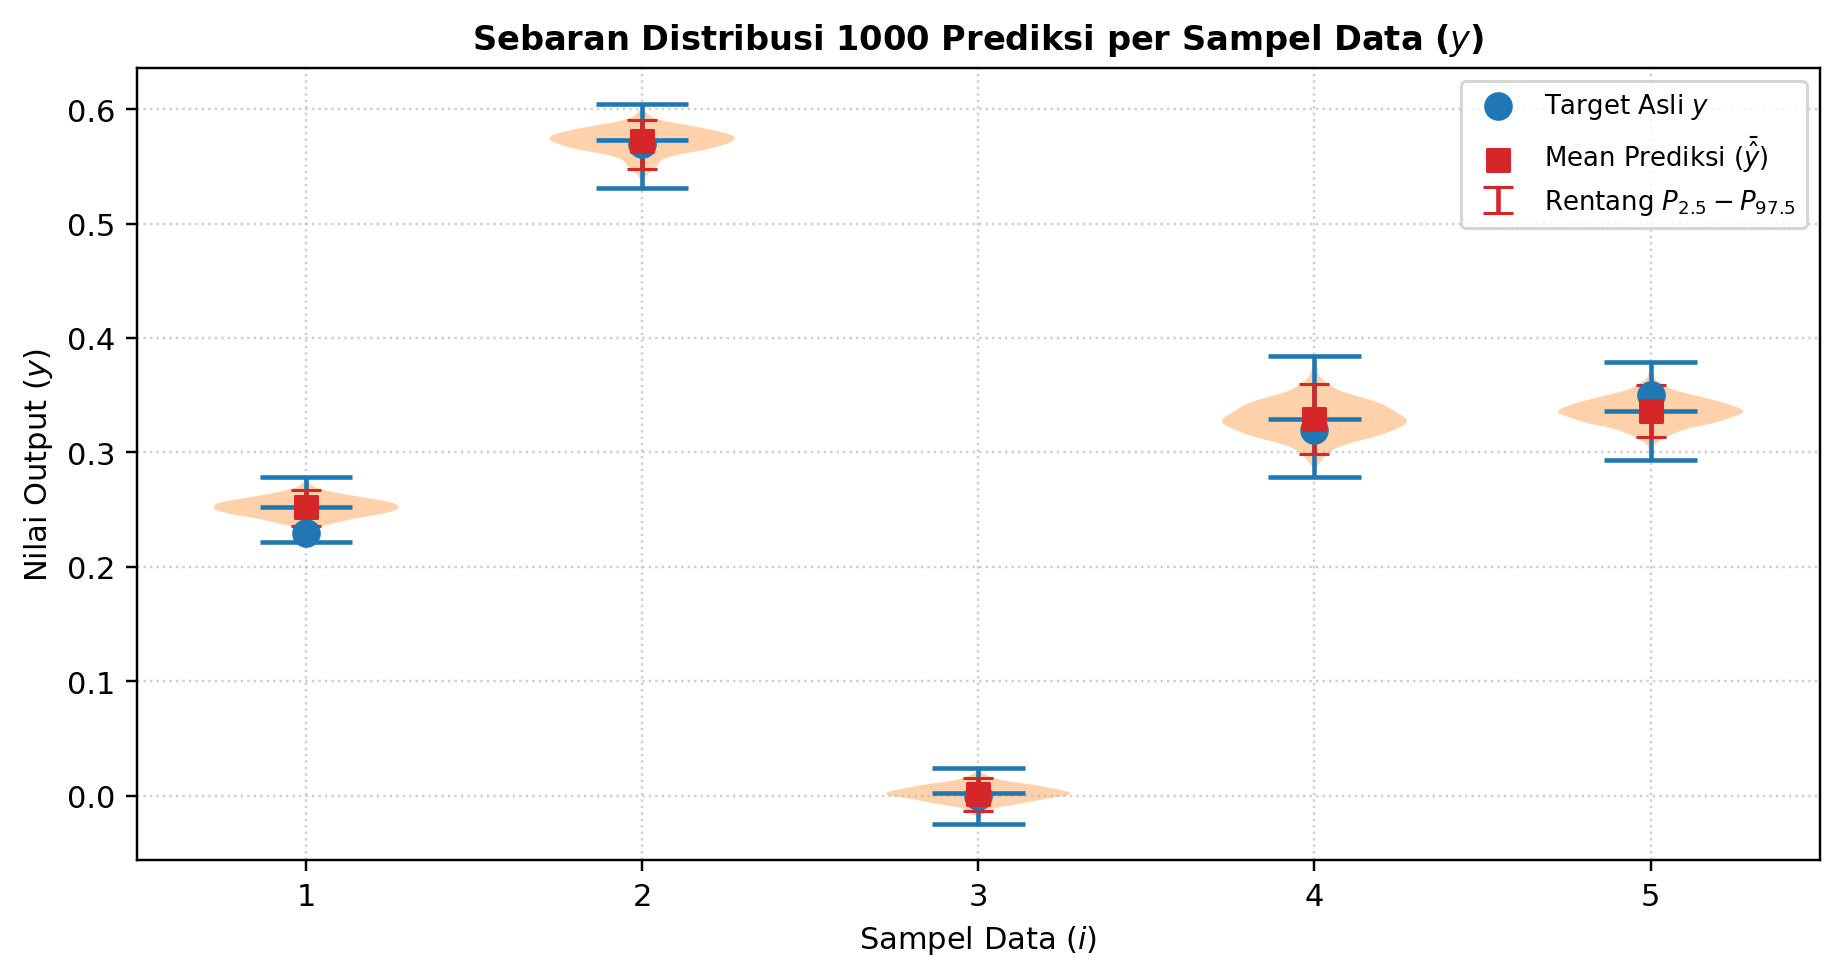
\includegraphics[width=0.72\textwidth]{r3_r1_fig1_distribusi.png}
    \caption{Grafik 1: Sebaran Distribusi 1000 Prediksi per Sampel Data.}
    \label{fig:r1_fig1}
\end{figure}

\begin{figure}[H]
    \centering
    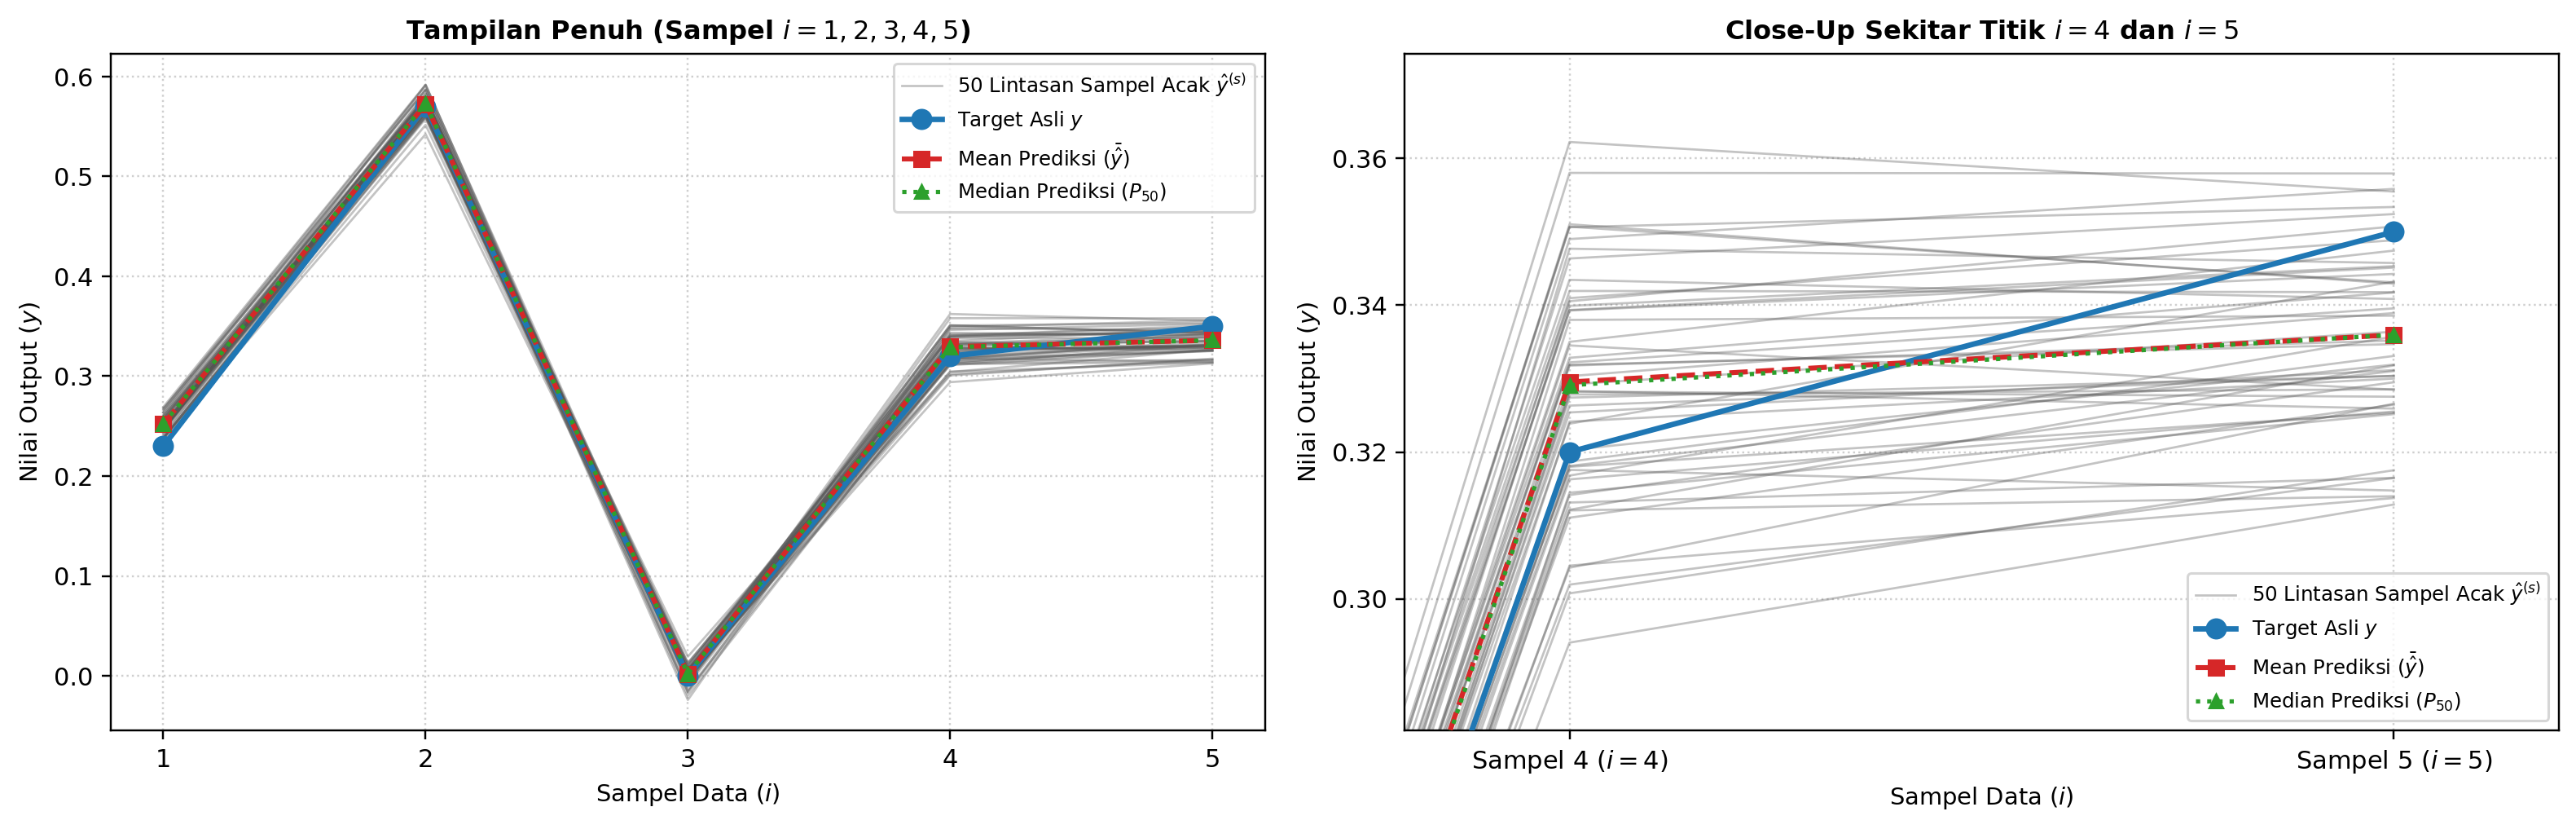
\includegraphics[width=0.96\textwidth]{r3_r1_fig2_lintasan.png}
    \caption{Grafik 2: Prediksi 1000 Sampel $Z$ dengan Plot 50 Lintasan Sampel Acak (Full vs Close-Up Titik 4 \& 5).}
    \label{fig:r1_fig2}
\end{figure}

\begin{figure}[H]
    \centering
    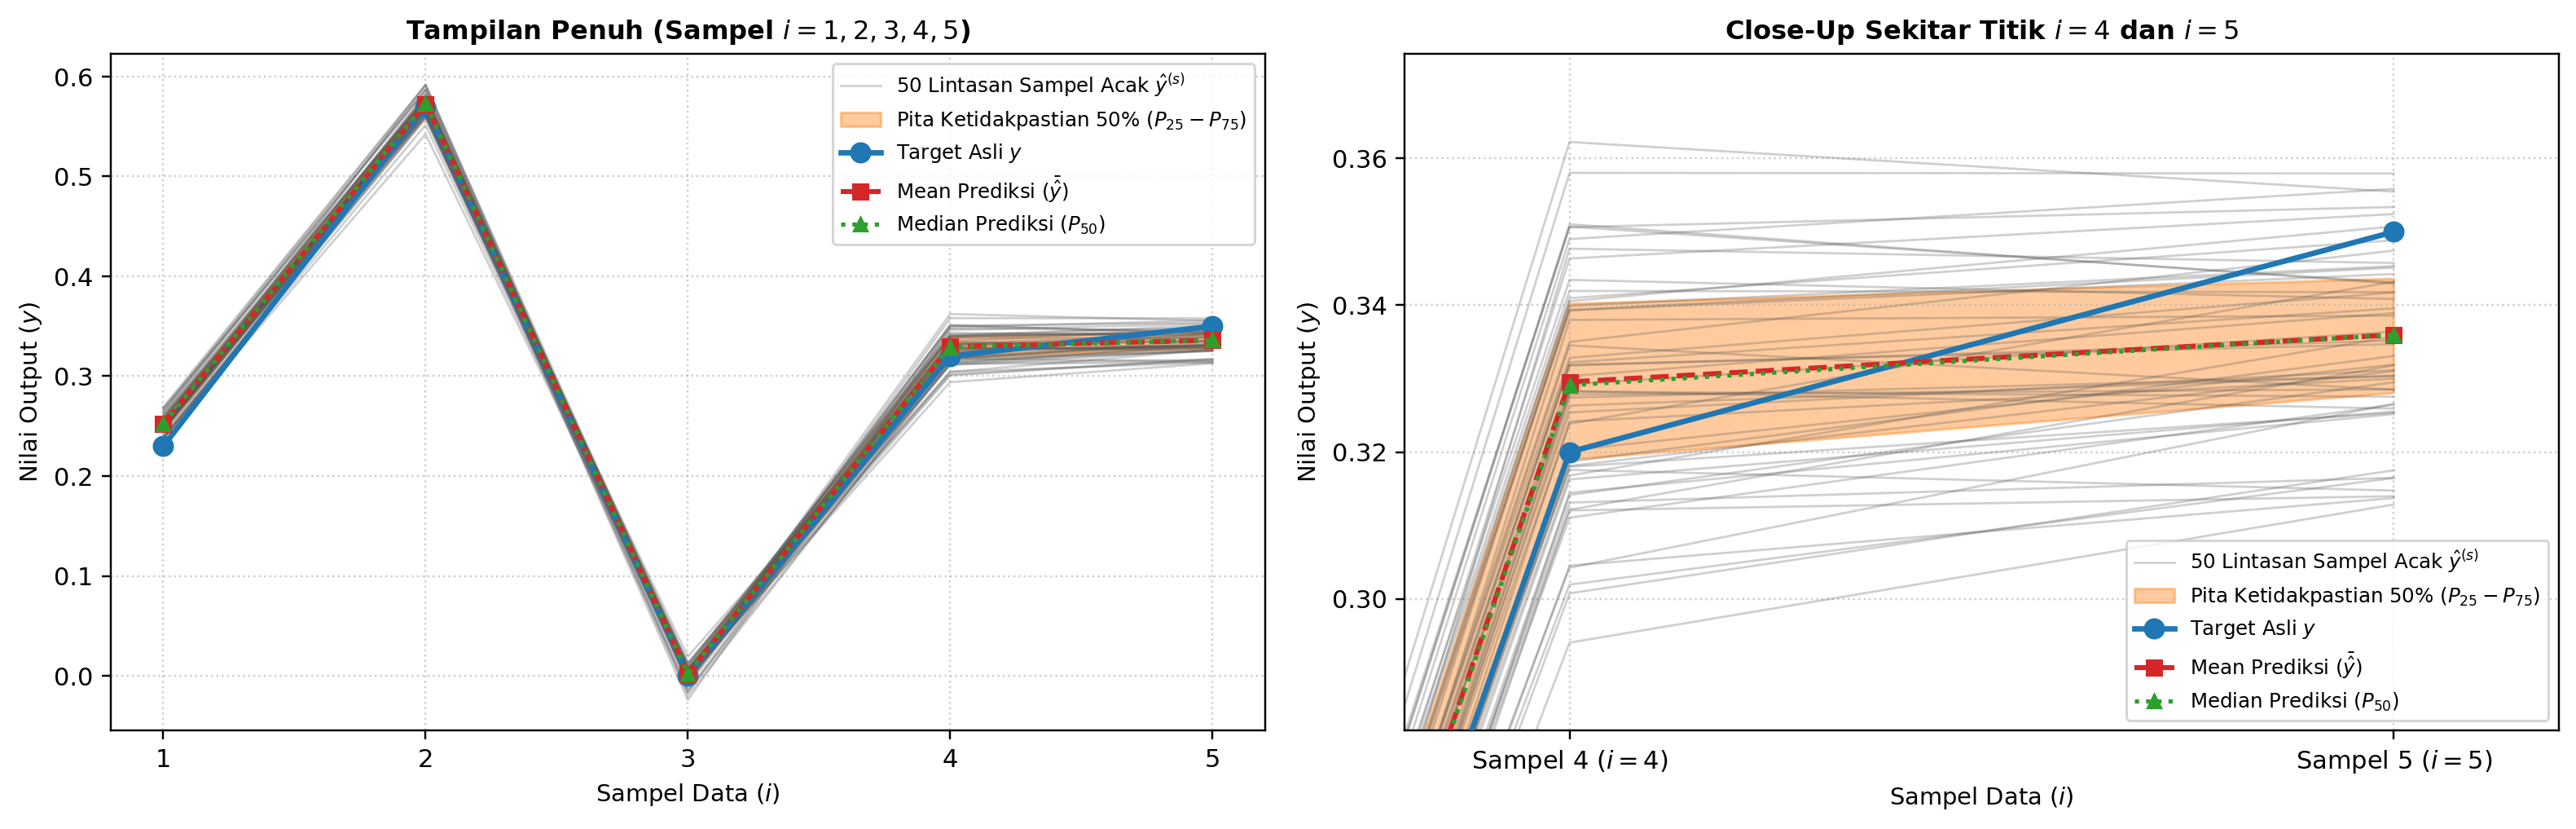
\includegraphics[width=0.96\textwidth]{r3_r1_fig3_pita50.png}
    \caption{Grafik 3: Prediksi 1000 Sampel $Z$ + 50 Lintasan Acak dengan Pita Ketidakpastian $50\%$ ($P_{25} - P_{75}$).}
    \label{fig:r1_fig3}
\end{figure}

\begin{figure}[H]
    \centering
    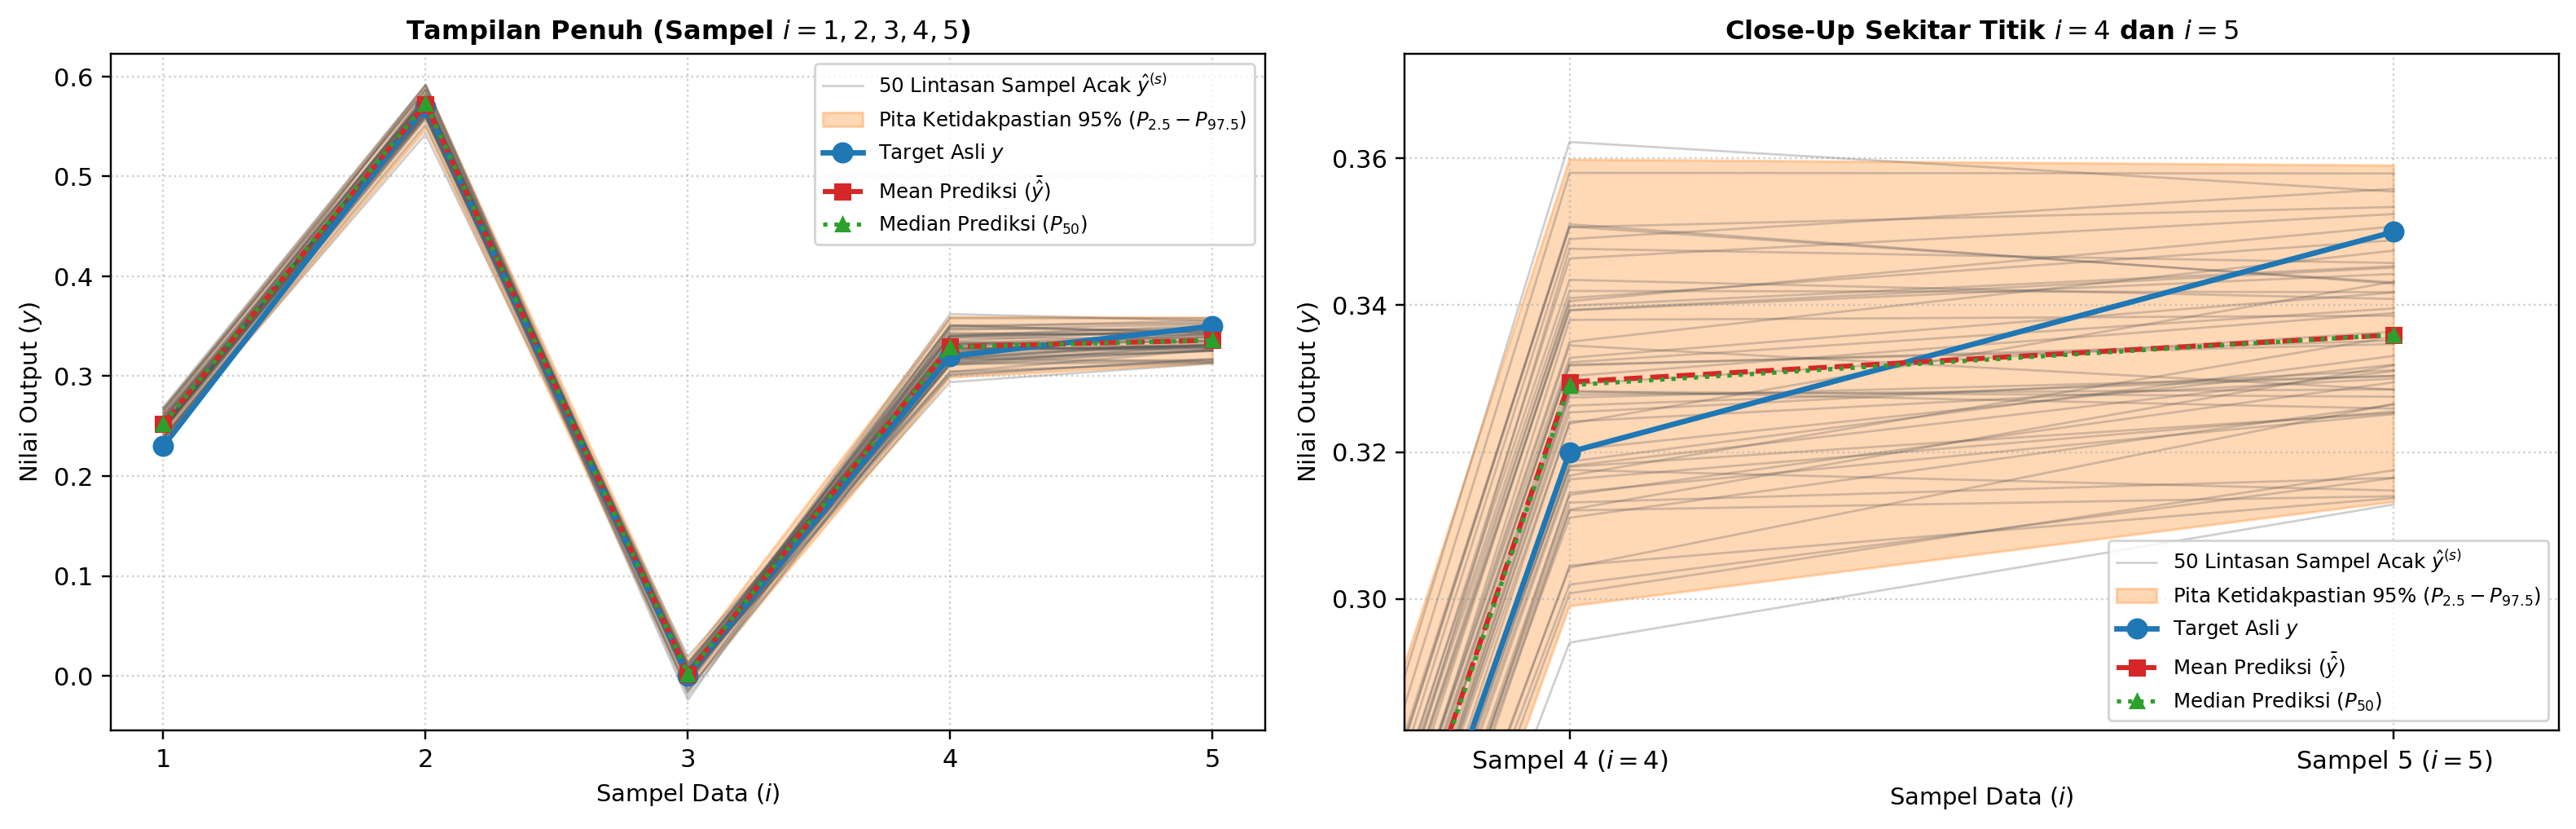
\includegraphics[width=0.96\textwidth]{r3_r1_fig4_pita95.png}
    \caption{Grafik 4: Prediksi 1000 Sampel $Z$ + 50 Lintasan Acak dengan Pita Ketidakpastian $95\%$ ($P_{2.5} - P_{97.5}$).}
    \label{fig:r1_fig4}
\end{figure}

% =========================================================================
% 3. EVALUASI WAKTU KOMPUTASI
% =========================================================================
\section{Evaluasi Waktu Komputasi}
\label{sec:waktu_komputasi}

\begin{table}[H]
    \centering
    \small
    \caption{Waktu Komputasi (\textit{Execution Time}) Pelatihan, Forward Pass 1000 Sampel $Z^{(\ell)}$, dan Perhitungan Persentil ($\mathbb{R}^3 \to \mathbb{R}^1$).}
    \label{tab:waktu_komputasi}
    \begin{tabularx}{\textwidth}{l >{\centering\arraybackslash}X}
        \toprule
        \textbf{Tahapan Komputasi} & \textbf{Waktu Proses ($\mathbb{R}^3 \to \mathbb{R}^1$)} \\
        \midrule
        1. Waktu Training ($T = 500$ Iterasi, Forward + Backward) & $85.4536\text{ ms}$ ($0.0855\text{ s}$) \\
        2. Waktu Forward Pass $S = 1000$ Sampel $Z^{(\ell)}$ & $54.3476\text{ ms}$ ($0.0543\text{ s}$) \\
        \quad $\hookrightarrow$ Rata-rata Waktu per $1\times$ Forward Pass ($\bar{t}_{\text{pass}} = t_{\text{forward}} / 1000$) & $0.0543\text{ ms / pass}$ \\
        3. Waktu Perhitungan Statistik ($\bar{\hat{y}}_i, s_{\hat{y}, i}$) \& Persentil & $8.9189\text{ ms}$ ($0.0089\text{ s}$) \\
        \midrule
        Total Waktu Forward Pass 1000 Sampel + Persentil & $63.2665\text{ ms}$ ($0.0633\text{ s}$) \\
        \bottomrule
    \end{tabularx}
\end{table}

\end{document}
